\documentclass[12pt,letterpaper]{hmcpset}
\usepackage[margin=1in]{geometry}
\usepackage{graphicx}
\usepackage{enumitem} % enumerate
\newcommand{\vb}{\mathbf}
% example usage of amssymb: $\mathbb{Z}$
% amsmath is loaded.

% info for header block in upper right hand corner
\name{}
\class{Math 19 - }
\assignment{Homework \#11}
\duedate{11/5/2019}

\begin{document}

\problemlist{Colley 3.1.3, 3.1.10, 3.1.17, 3.2.10, \\ 3.3.9, 3.3.18, 3.4.4, 3.4.12(b)(c), 3.4.13, 3.4.16}

\begin{problem}[Colley 3.1.3]
  Sketch the images of the following path, using arrows to indicate the direction in which the parameter increases:
  \[\begin{cases}
      x = t\cos t \\
      y = t\sin t
    \end{cases}, -6\pi \leq t \leq 6\pi \]
\end{problem}
\clearpage

\begin{problem}[Colley 3.1.10]
  Calculate the velocity, speed, and acceleration of the path:
  \[ \vb x(t) = \left(e^t, e^{2t}, 2e^t \right) \]
\end{problem}
\clearpage

\begin{problem}[Colley 3.1.17]
  Find an equation for the line tangent to the given path at the indicated value for the parameter:
  \[ \vb x(t) = \left(t^2, t^3, t^5\right),\quad t=2 \]
\end{problem}
\clearpage

\begin{problem}[Colley 3.2.10]
  If $f$ is a continuously differentiable function, show how Definition 2.1 may be used to established the formula
  \[ L = \int_a^b\sqrt{1 + (f'(x))^2}~dx \]
  \textbf{Definition 2.1:} The \textbf{length} $L(\vb x)$ of a $C^1$ path $\vb x:[a, b]\to \vb R^n$ is found by integrating its speed: \[ L(\vb x) = \int_a^b ||\vb x'(t)||~dt \]
\end{problem}
\clearpage

\begin{problem}[Colley 3.3.9]
  Sketch the given vector field on $\vb R^3$:
  \[ \vb F = (0, z, -y) \]
  In addition to the sketch, provide a description of the vector field.
\end{problem}
\clearpage

\begin{problem}[Colley 3.3.18]
  Verify that the path given is a flow line of the indicated vector field.
  Justify the result geometrically with an appropriate sketch.
  \[ \vb x(t) = (\sin t, \cos t, 2t), \quad \vb F = (y, -x, 2) \]
\end{problem}
\clearpage

\begin{problem}[Colley 3.4.4]
  Calculate the divergence of the vector field given:
  \[ \vb F = z\cos\left(e^{y^2}\right)\vb i + x\sqrt{z^2 + 1}\vb j + e^{2y}\sin 3x\vb k \]
\end{problem}
\clearpage

\begin{problem}[Colley 3.4.12(b)(c)]
  \begin{enumerate}[label=(\alph*)]
    \addtocounter{enumi}{1}
  \item Use geometry to determine $\nabla \times \vb F$, where $\vb F = \frac{(x\vb i + y\vb j + z\vb k)}{\sqrt{x^2 + y^2 + z^2}}$.
  \item For $\vb F$ as in part (b), verify your intuition by explicitly computing $\nabla \times \vb F$.
  \end{enumerate}
\end{problem}
\clearpage

\begin{problem}[Colley 3.4.13]
  Can you tell in what portions of $\vb R^2$, the vector fields shown in Figures 3.43-3.46 have positive divergence? Negative divergence?
\end{problem}
\begin{figure}[h]
  \begin{minipage}{0.49\textwidth}
  \centering
    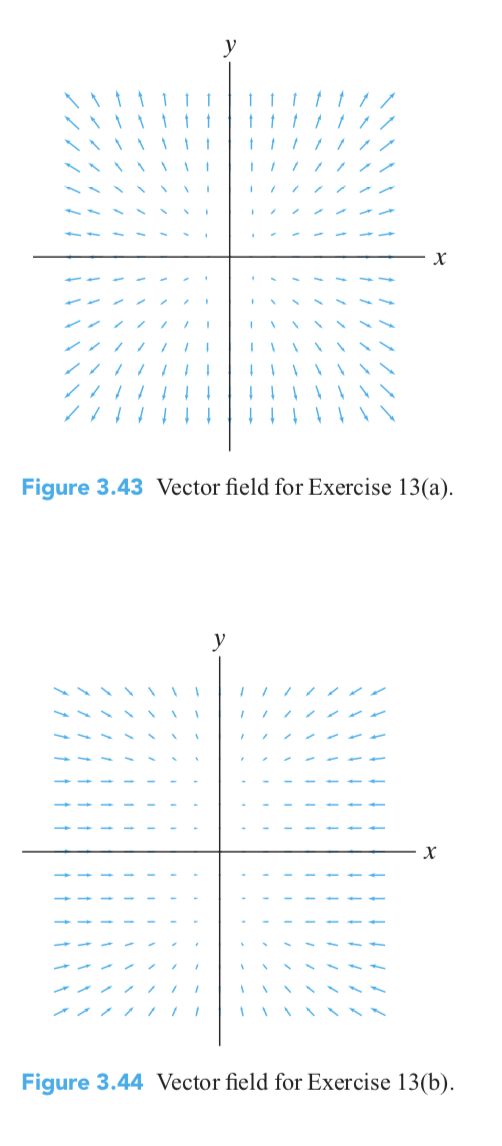
\includegraphics[width=0.6\textwidth]{assets/11_1.png}
    % \caption{\label{fig:1}}
  \end{minipage}
  \begin{minipage}{0.49\textwidth}
    \centering
    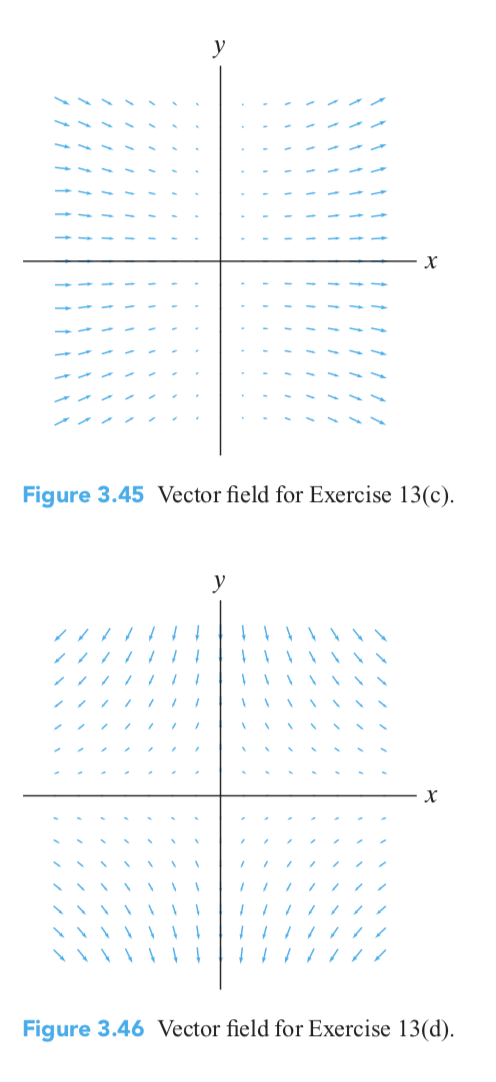
\includegraphics[width=0.6\textwidth]{assets/11_2.png}
    % \caption{\label{fig:2}}
  \end{minipage}
\end{figure}
\clearpage

\begin{problem}[Colley 3.4.16]
  Prove Theorem 4.4. \\
  
  \textbf{Theorem 4.4:} Let $F: X \subseteq \vb R^3 \to \vb R^3$ be a vector field of class $C^2$.
  Then $\text{div } (\text{curl } \vb F) = 0$. That is, curl $\vb F$ is an incompressible vector field.
\end{problem}

\end{document}
